\chapter{Arquitectura de la Game Boy Advance}\label{sec:arquitectura}

Con un procesador RISC como corazón del sistema, la Game Boy Advance tiene unas especificaciones modestas, similares a lo que veríamos en los dispositivos embebidos de hoy en día. El dispositivo cuenta con un unidad ARM7TDMI de 32 bits como procesador principal. Tiene también un coprocesador el cual fue utilizado en la iteración anterior de la consola, el Sharp SM83 (basado en el set de instrucciones 8080 de 8 bits). Esto permite a la consola jugar, de forma nativa, a juegos desarrollados para la Game Boy original \cite{bib:rodrigo}. 

Estos dos procesadores residen en el mismo SoC (véase en la Figura \ref{fig:circuit}) y permiten a la consola ejecutarse en varios modos. Podemos distinguir los siguientes:
\begin{itemize}
\item El \textbf{modo ARM}, que hace que el procesador funcione a 16.78 MHz, manejando instrucciones de 32 bits.
\item El \textbf{modo THUMB}, reservado para optimizar partes del código. En este modo la consola también funciona a una frecuencia de 16.78 MHz, pero solo acepta instrucciones de 16 bits.
\item El \textbf{modo CGB} (Color Game Boy), que utiliza el coprocesador mencionado anteriormente para ejecutar código escrito para la Game Boy Color original (la frecuencia puede variar entre 4.2 MHz y 8.4MHz).
\item El \textbf{modo DMG} (Dot Matrix Game), similar el modo anterior, aunque esta vez limitado a 4.2 MHz. Está reservado para su uso en juegos programados para la Game Boy con pantalla monocromática.
\end{itemize}

\begin{figure}[t]
    \centering
    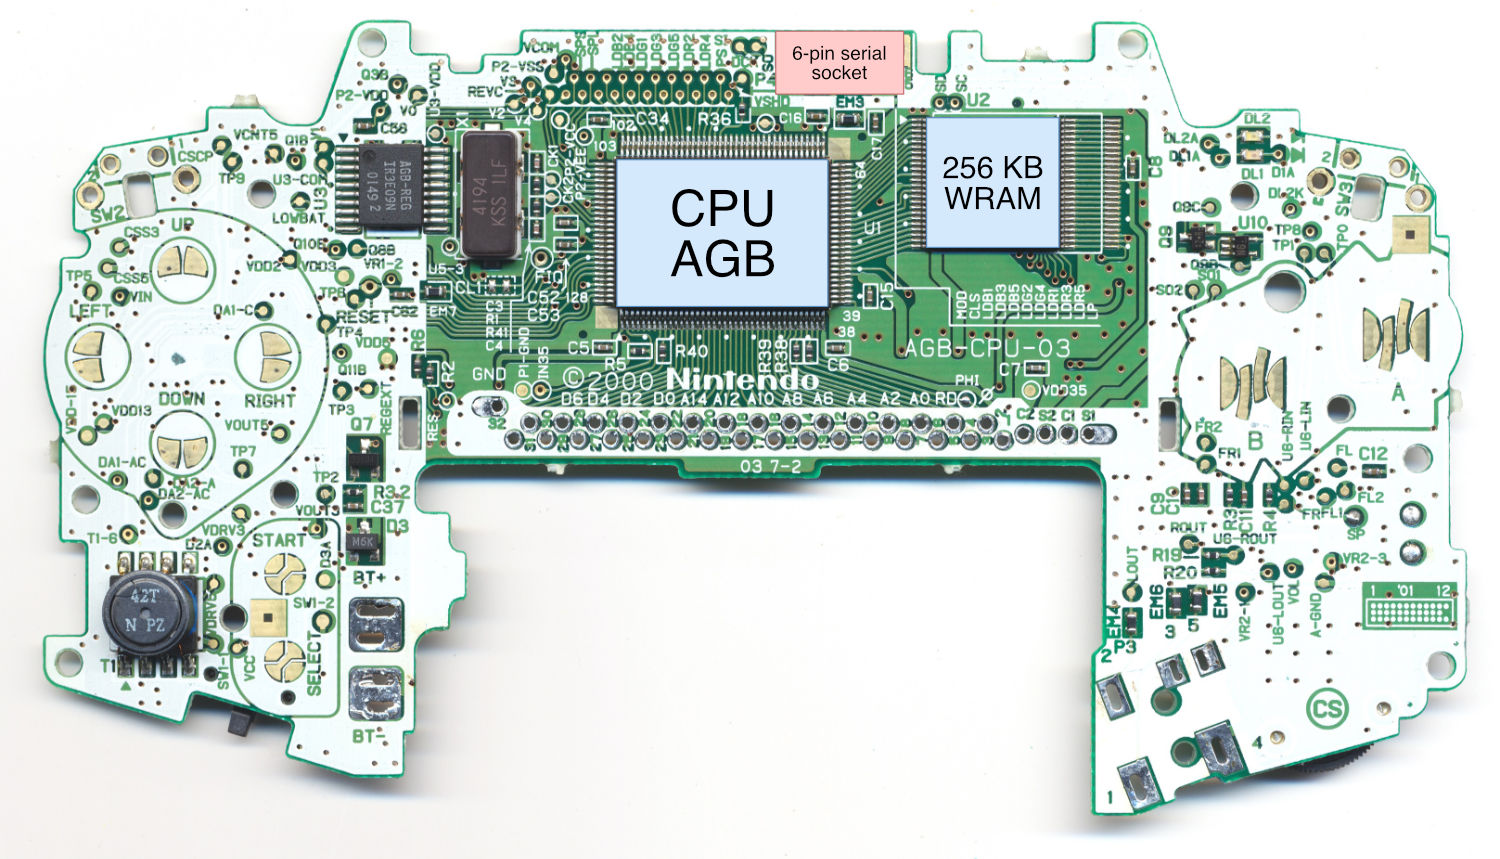
\includegraphics[width=.8\textwidth]{capitulos/capitulo2/circuit.jpg}
    \caption{El circuito de la Game Boy Advance \cite{bib:rodrigo}.}
    \label{fig:circuit}
\end{figure}


Es importante mencionar que ambos procesadores no pueden ejercer la función de procesador central simultáneamente. Por ende, el programador puede cambiar del modo ARM al THUMB y viceversa, pero no de un modo que use el procesador ARM7 a otro que utilice el Sharp SM83 \cite{bib:gbatek}.

La consola cuenta con el mapa de memoria detallado en la Tabla~\ref{tab:mapa} que, dependiendo a que sección se accede, tiene buses de 32, 16 u 8 bits. La práctica de tener buses de diferentes tamaños es común en consolas, incluso de sobremesa como la PlayStation 2~\cite{bib:comp_arch_quant}.

\begin{table}[h]
	\centering
	\begin{tabular}{| l | l | l | l |}
		\hline
		\textbf{Nombre} & \textbf{Sección} & \textbf{Tamaño} & \textbf{Bus} \\ \hline
		ROM del sistema & 0x00000000-0x00003FFF & 16 KB & 32 bits \\ \hline
		RAM externa (On-board RAM) & 0x02000000-0x0203FFFF & 256 KB\tablefootnote{A pesar de tener disponible 256 KB, la Game Boy reserva en los últimos 256 bytes datos que gestiona internamente, como el vector de interrupciones.} & 16 bits\\ \hline
		RAM interna (On-chip RAM) & 0x03000000-0x03007FFF & 32 KB & 32 bits \\ \hline
		RAM de IO & 0x04000000-0x040003FE & - & 32 bits \\ \hline
		RAM de paleta & 0x05000000-0x050003FF & 1 KB & 16 bits \\ \hline
		VRAM & 0x06000000-0x06017FFF & 96 KB & 16 bits \\ \hline
		Memoria de objetos & 0x07000000-0x070003FF & 1 KB & 32 bits \\ \hline
		ROM y flash del cartucho & 0x08000000-0x0DFFFFFF & $\leq$ 96 MB  & 16 bits \\ \hline
		SRAM del cartucho & 0x0E000000-0x0E00FFFF & $\leq$ 64 KB & 8 bits \\ \hline
	\end{tabular}
	\caption{Mapa de memoria de la Game Boy Advance.}
	\label{tab:mapa}
\end{table}


Los espacios que aparecen en la tabla anterior, entre la ROM del sistema y la RAM externa (en concreto, 0x00004000-0x01FFFFFF), son regiones que no se utilizan o en las que el programador no tiene que intervenir de ninguna manera \cite{bib:gba_manual}.

A continuación, comentaremos brevemente la función que se le da a cada sección.

\begin{itemize}
	\item \textbf{ROM del sistema}: Encabezando el mapa de memoria de la consola encontramos la ROM del sistema, la cual guarda, como su nombre indica, código inmutable del sistema. Contiene por ejemplo la BIOS y rutinas que el programador puede utilizar en su juego. Entre las rutinas incluidas se pueden distinguir algunas para calcular operaciones  aritméticas complejas y transformaciones afines, y otras para llevar a cabo funciones de descompresión, sonido, copia de memoria e interacción con otras consolas al conectarlas mediante el cable \textit{link}\footnote{La Game Boy Advance permitía jugar con hasta 4 personas mediante una conexión por cable.} (función conocida como \textit{multi-boot}).
	\item \textbf{RAM}: A continuación, después de la ROM, se encuentra la RAM de la consola (también conocida como EWRAM o External Work RAM), en la que se distinguen dos tipos. La primera región, posicionada en la dirección 0x02000000, reside fuera del SoC (véase la Figura \ref{fig:circuit}). Cuenta con un tamaño de 256 KB y un bus de 16 bits por el cual podemos considerar esta sección como la RAM ``lenta''. La siguiente región que encontramos en el mapa de memoria, la RAM interna, ofrece un bus completo de 32 bits, pero con un tamaño reducido (comparado con la RAM externa) de 32 KB. En la Figura \ref{fig:distribucion_1} se muestra la distribución y localización de la IWRAM y EWRAM. \\

	\begin{figure}[h]
	    \centering
	    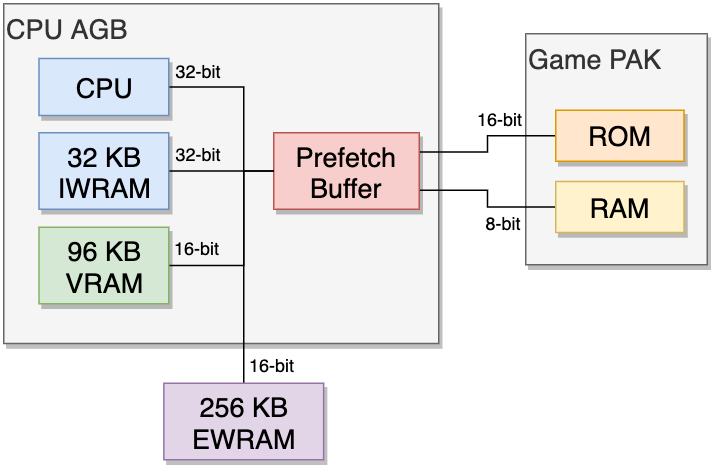
\includegraphics[width=.5\textwidth]{capitulos/capitulo2/distribucion.png}
	    \caption{Distribución de la memoria de la Game Boy Advance \cite{bib:rodrigo}.}
	    \label{fig:distribucion_1}
	\end{figure}

	\item \textbf{Registro de control de entrada y salida}: En la siguiente sección aparece ``mapeado'' el registro de control de entrada y salida en el que el programador puede consultar información (como las teclas que el usuario presiona) y modificar la configuración de la consola. Por ejemplo, en esta región se encuentran los valores que determinarán el tipo de gráficos que utilizará el juego.
	\item \textbf{RAM de paleta}: La RAM de paleta, o ``palette RAM'' en inglés, es la sección de memoria que cubre el espacio necesario para albergar las paletas de colores de los diferentes modos de vídeo y gráficos disponibles.
	\item \textbf{VRAM}: En la VRAM se almacenan los índices de la paleta de colores para referenciarlos. Además de esta función en algunos modos de la Game Boy Advance, la VRAM también contiene los objetos o píxeles que aparecerán en pantalla. Más adelante se darán más detalles.
	\item \textbf{Memoria de Objetos}: La memoria de objetos (OAM, de "Object Attribute Memory" en inglés), al igual que la RAM de paleta, se utiliza en unos modos concretos y se encarga de guardar los datos de objetos a mostrar, informalmente nombrados por el anglicismo {\it sprites}. Estos ``objetos'' son, normalmente, el texto y personajes que aparecen en los juegos 2D. Algunos de los atributos que maneja esta región son la posición, rotación, escala y tamaño. \\

	Las tres secciones descritas, RAM de paleta, VRAM y OAM, forman parte de la PPU (\textit{Picture Processing Unit}) de la Game Boy Advance. Esta se encarga de combinar y procesar la información almacenada en dichas regiones (qué información procesa  y cómo dependerá del modo de vídeo utilizado) para crear una imagen que el usuario pueda ver. La distribución de la PPU se observa en la Figura \ref{fig:distribucion_2}.

	\begin{figure}[h]
	    \centering
	    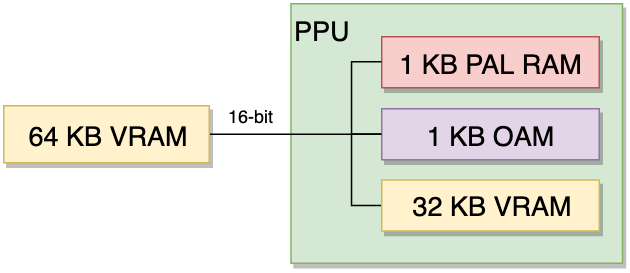
\includegraphics[width=.5\textwidth]{capitulos/capitulo2/ppu.png}
	    \caption{La PPU de la Game Boy Advance.}
	    \label{fig:distribucion_2}
	\end{figure}

	\item \textbf{ROM y SRAM del cartucho}: La última región en el mapa de memoria es la vinculada con el cartucho del juego, que se introduce en la ranura que ofrece la consola y funciona mediante una conexión paralela. La ejecución del juego empieza en esta dirección de memoria\footnote{Salvo en juegos multijugador, en ese caso la ejecución del juego comienza en las instrucciones localizadas en la RAM externa (0x02000000).}, la ROM del cartucho (0x08000000). Para que los jugadores puedan guardar sus partidas se dedican los últimas 64 KB, sección denominada SRAM \cite{bib:tonc,bib:gba_manual,bib:gbatek}.
\end{itemize}

Todas las zonas de memoria anteriores se pueden ver distribuidas en el diagrama del circuito de la consola, en la Figura \ref{fig:diagrama}.

\begin{figure}[h]
    \centering
    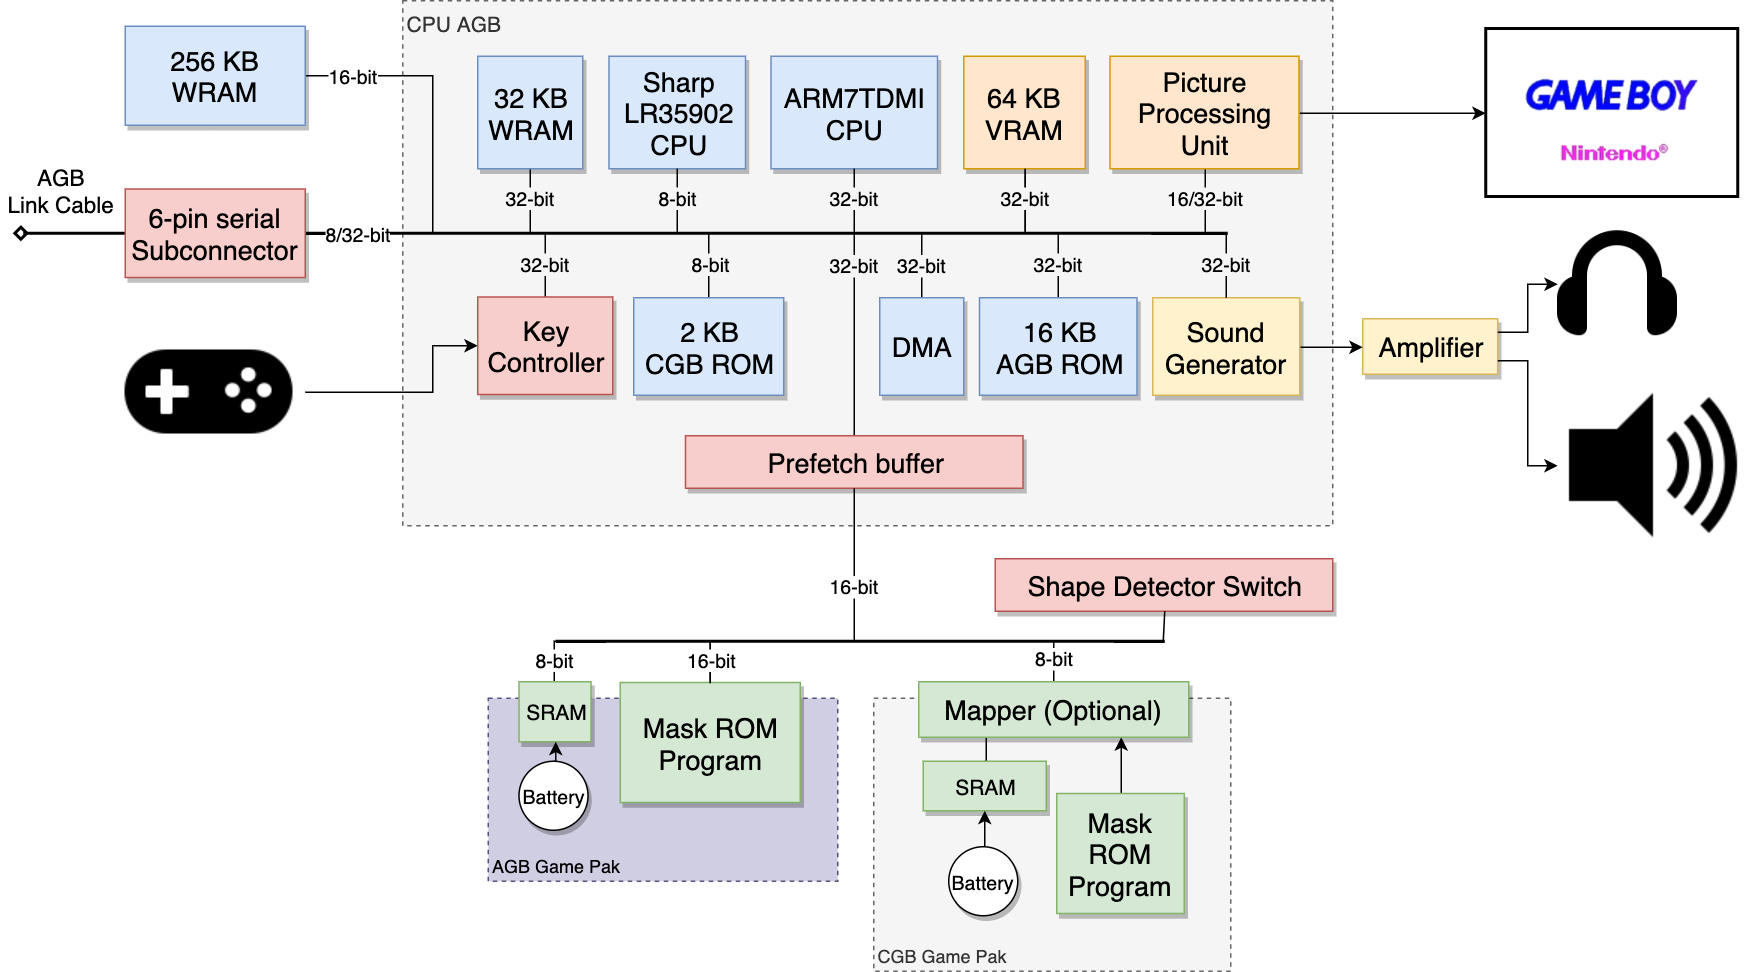
\includegraphics[width=.9\textwidth]{capitulos/capitulo2/diagram.png}
    \caption{Diagrama simplificado del circuito de la Game Boy Advance \cite{bib:rodrigo}.}
    \label{fig:diagrama}
\end{figure}
\FloatBarrier{}

\section{Procesador ARM7TDMI}
En este punto se incluyen los aspectos más importantes del procesador principal de la Game Boy Advance. Toda la información se puede encontrar en \cite{bib:arm} (el documento de referencia del procesador), complementada con detalles adicionales sobre el juego de instrucciones utilizado en \cite{bib:armv4_isa}.

Para cumplir con las exigencias de potencia computacional de la nueva generación de consolas portátiles, Nintendo, decidió diseñar un procesador basado en ARMv4, un  juego de instrucciones (ISA o \textit{Instruction Set Architecture} en inglés)  RISC. Las especificaciones del ISA nos dan una idea de las características del dispositivo:

\begin{itemize}
	\item \textbf{ARMv4} tiene un total de 37 registros de 32 bits, de los cuales 31 son generales y 6 son de estado. En la Game Boy existen diferentes modos. Cada uno de ellos tiene acceso a 17, o menos, de los registros disponibles. El acceso según el modo del procesador a los registros del sistema se describe en la Figura \ref{fig:registros_arm}. Es importante resaltar que, tal y como pasa con otros procesadores ARM, algunos de los 37 registros no son \textit{banked registers}, lo que significa que varios modos compartirán registros y, por lo tanto, los valores de estos pueden ser sobrescritos. \\

	Ignorando los modos privilegiados mostrados en la Figura \ref{fig:registros_arm} (\textit{FIQ, Supervisor, Abort, IRQ, Undefined}), los usos de los registros en el modo general (primera columna de la figura, \textit{System and User}) que controlará el programador son:

		\begin{itemize}
			\item Generales: Los registros considerados como generales son R0-R12. Sin embargo, mientras que el modo ARM tiene libertad total para acceder a cada uno de los 13, el modo THUMB solo puede acceder de R8 a R12 utilizando instrucciones específicas. 
			\item \textit{Stack Pointer}: El registro R13 se utiliza para guardar la dirección de la pila, esto se realiza por convención en el modo ARM, dado que también se puede utilizar como un registro de uso general. No obstante, en el caso del modo THUMB debe utilizarse como \textit{Stack Pointer}.
			\item \textit{Link Register} y \textit{Program Counter}: R14 se reserva para guardar la dirección de memoria de R15 (\textit{Program Counter}) al realizar una instrucción de salto, también conocida como instrucción de \textit{branch}. No obstante, como ocurre con el registro R13, en caso de no usar este tipo de instrucciones, el modo ARM permite utilizar el registro para uso general. Otra diferencia a tener en cuenta entre los dos modos es el valor del contador del programa, el registro R15, que almacena el valor del contador en los bits 2-31 en el modo ARM y 1-31 en el modo THUMB.
			\item CPSR y SPSR: El registro CPSR (\textit{Current Program Status Register}), accesible en todos los modos, almacena datos como el estado del procesador e información de control como el resultado de instrucciones CMP. En los modos privilegiados encontramos un registro adicional además de los 17 registros explicados en el punto anterior, denominado SPSR (\textit{Saved Program Status Register}), en el que se guardan los valores del registro CPSR en caso de excepción.
		\end{itemize}

\begin{figure}[t]
    \centering
    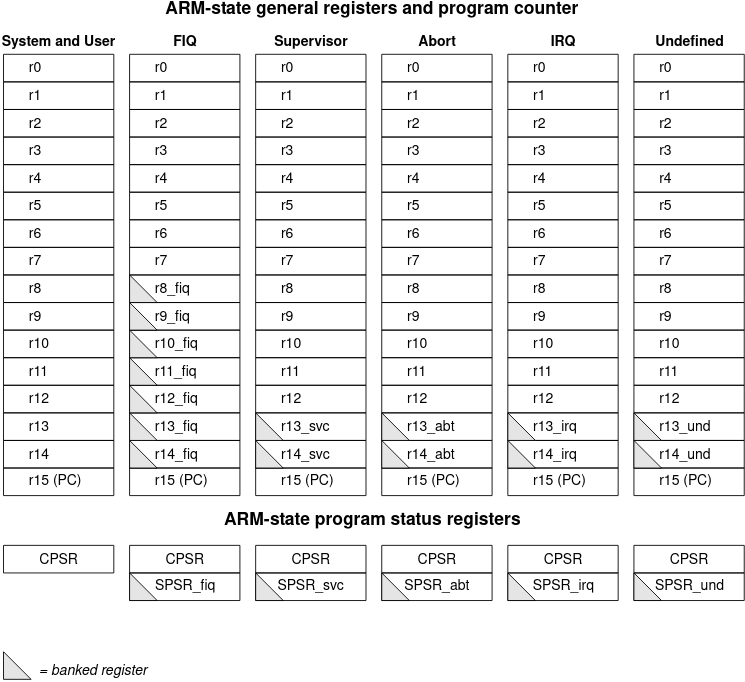
\includegraphics[width=.8\textwidth]{capitulos/capitulo2/registros.png}
    \caption{Registros por modo del procesador ARM7TDMI.}
    \label{fig:registros_arm}
\end{figure}

Las limitaciones que se comentaron anteriormente con el modo THUMB del procesador y los efectos que tiene en el acceso de los registros quedan representados en la Figura \ref{fig:registros_thumb}.

\begin{figure}[h]
    \centering
    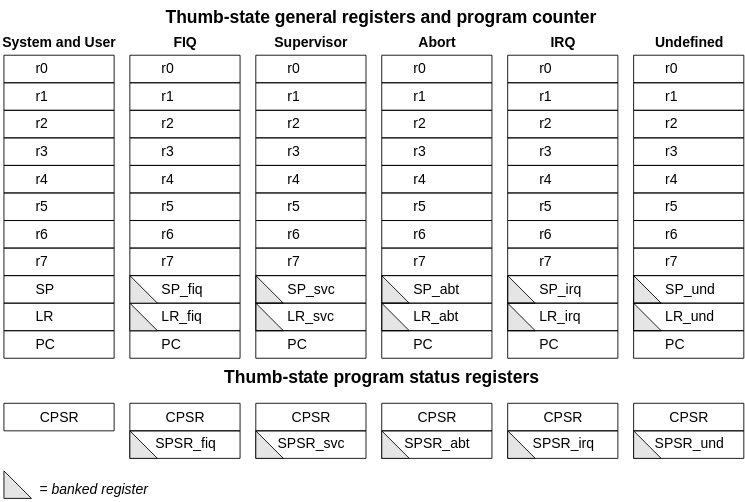
\includegraphics[width=.8\textwidth]{capitulos/capitulo2/registros_thumb.png}
    \caption{Registros por modo del procesador ARM7TDMI cuando este utiliza el set de instrucciones THUMB.}
    \label{fig:registros_thumb}
\end{figure}

\item La consola utiliza un juego de instrucciones \textbf{load-store} en el cual todas las operaciones aritméticas que operan en memoria tienen que realizarse mediante instrucciones load. Este \textit{ISA} permite también el uso de constantes de 8, 12 y 24 bits para minimizar el uso de instrucciones.
\end{itemize}

Una vez que se han comentado las características del conjunto de instrucciones, se pasa a describir las características específicas del ARM7TDMI. Entre las más destacables se encuentran:

\begin{enumerate}
	\item Un camino de datos segmentado de tres etapas: \textit{Fetch}, \textit{Decode} y \textit{Execute} (véase la Figura \ref{fig:pipeline}). En concreto, esta implementación de la segmentación para el ARM7TDMI permite ejecutar hasta tres instrucciones de forma concurrente.

		\begin{figure}[h]
		    \centering
		    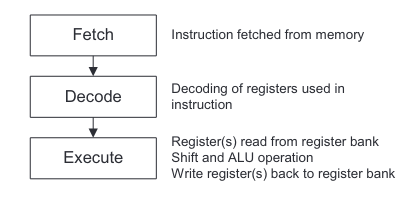
\includegraphics[width=.5\textwidth]{capitulos/capitulo2/pipeline.png}
		    \caption{Segmentación de instrucciones de la Game Boy Advance.}
		    \label{fig:pipeline}
		\end{figure}

	\item Una ALU de 32 bits, mejorando de forma sustancial las capacidades de modelos anteriores. De esta forma, la consola podía operar con números de 32 bits sin tener que consumir ciclos adicionales del procesador.
	\item Un procesador con extensiones específicas, las cuales aparecen en el propio nombre, ARM7\textbf{TDMI}. A continuación se detallan:

		\begin{itemize}
			\item \underline{\textbf{T}}humb: Tal y como se indicó previamente, el procesador soporta un modo que opera con instrucciones de 16 bits. Al ejecutarse en el hardware, las instrucciones se descomprimen a instrucciones de 32 bits sin pérdida de rendimiento. Según las estimaciones de ARM, programar en el modo THUMB reduce el tamaño del programa un 35\% (comparado con el modo ARM) y proporciona un rendimiento del 160\% al utilizarse en sistemas que trabajan en 16 bits \cite{bib:arm}. Todas las mejoras mencionadas anteriormente son posibles siempre y cuando las limitaciones que implica el modo (el limitado acceso a los registros superiores, R8-R12, por ejemplo) no supongan un inconveniente al programar.
			\item Extensiones de \underline{\textbf{D}}epuración mediante JTAG: \textit{Joint Test Access Group} o \textit{Standard Test Access Port and Boundary-Scan Architecture}, siendo este último el nombre oficial dado por la IEEE. Se trata de una especificación que permite a partir de una conexión, depurar un microcontrolador directamente en el hardware.
		\item \underline{\textbf{M}}ultiplicador mejorado: Los ciclos necesarios para completar multiplicaciones con números de 32 bits se reducen de forma considerable con respecto a las versiones anteriores del procesador.
		\item Embedded\underline{\textbf{I}}CE macrocell: Con ICE, \textit{In-circuit emulation} en inglés, la consola añade la posibilidad de manipular directamente el hardware del dispositivo para poder realizar una depuración a fondo del programa.
		\end{itemize}

		La distribución de la lógica necesaria para poder incluir las extensiones de depuración mediante JTAG y EmbeddedICE macrocell se puede observar en la Figura~\ref{fig:debug_block}. Aquí se puede ver también la adición de un controlador llamado ``TAP''. Este sirve de intermediario entre la interfaz serial JTAG y las \textit{scan chains}, que habilitan la comunicación entre la interfaz ICE y el procesador de la consola.

		\begin{figure}[h]
		    \centering
		    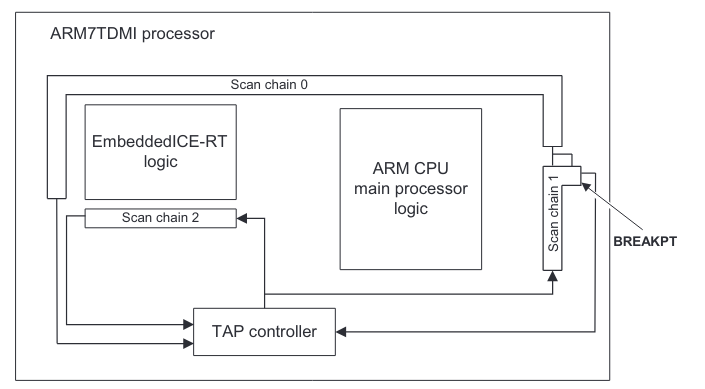
\includegraphics[width=.8\textwidth]{capitulos/capitulo2/debug_block.png}
		    \caption{Distribución del EmbeddedICE-RT y controlador TAP en el diagrama de bloques del ARM7TDMI.}
		    \label{fig:debug_block}
		\end{figure}
		\FloatBarrier{}

\end{enumerate}

El lector interesado puede consultar \cite{bib:arm} para obtener más información sobre el procesador ARM7TDMI.

\section{Coprocesador Sharp SM83}
Para mantener la retrocompatibilidad de modelos anteriores con la Game Boy Advance, Nintendo incluyó un coprocesador que se encargaría de llevar a cabo esta labor. Como era de esperar, la compañía incluyó el mismo procesador utilizado para la Game Boy original, un procesador Sharp SM83 dentro del SoC Sharp LR35902. El procesador, dependiendo del dispositivo, funcionaba a una frecuencia de 4.19 MHz u 8.38 MHz. Por aquel entonces, incluir el hardware de dispositivos anteriores era una práctica convencional, puesto que el hardware no era lo suficientemente potente como para emular generaciones pasadas. La situación hoy en día es diferente según el caso. Por ejemplo, la Xbox One ya incluye un emulador para poder ejecutar juegos de Xbox 360\footnote{https://www.extremetech.com/gaming/257851-microsoft-built-xbox-360-xbox-compatibility-xbox-one}. 

La información disponible sobre el procesador Sharp es escasa. No obstante, se sabe que su diseño se basa, fundamentalmente, en los procesadores \textbf{Intel 8080} y \textbf{Zilog Z80}. A continuación se detallarán las características heredadas de cada uno de ellos.

La primera característica, que se hace evidente al saber en los dos procesadores en los que se basa, es que el \textbf{Sharp SM83 es un procesador de 8 bits}.

Sharp, al diseñar el procesador, combinó características de cada uno. Una de ellas sería la sintaxis utilizada al programar en ensamblador, en concreto, la sintaxis utilizada por el Z80. Esta se escogería seguramente por el \textit{copyright} que tenía Intel en su día sobre la sintaxis utilizada en el 8080. Por lo tanto, las diferencias encontradas son menores. Los únicos cambios son el de los nombres de instrucciones abreviadas que utilizaba Intel, que se reemplazaron por otras que usaban el nombre completo (por ejemplo, ``LOAD'' en vez de ``LD'').

En cuanto a registros se refiere, se tomó prestado el diseño utilizado en el Intel 8080, pero con ligeras modificaciones que destacaremos a continuación. En concreto, los \textbf{10 registros} que utiliza el procesador Sharp son:

\begin{itemize}
\item El registro A de 8 bits, reservado para el acumulador.
\item El registro F de 8 bits, reservado para guardar el estado del procesador.
\item El resto de registros (el B, C, D, E, H, y L) de 8 bits, diseñados para un uso general por parte del programador.
\item Los registros PC y SP, de 16 bits cada uno, se reservaban para su uso como contador de programa y puntero de pila, respectivamente.
\end{itemize}

Dado que algunas instrucciones lo permitían, se podían utilizar los registros en pares de la siguiente manera: AF, BC, DE y HL.

A pesar de tomar prestado el diseño de los registros, lo que \textbf{no heredó fue el esquema I/O del Intel 8080}, que permitía acceder a cada puerto mediante una instrucción específica. Se optó por el mismo sistema que utiliza la Game Boy Advance, ``mapeando'' cualquier puerto a una zona de memoria.

Otra especificación que copió del Intel 8080 fue el \textbf{bus de datos de 8 bits y direccionamiento de 16 bits}, con el cual se podían acceder a 64 KB de memoria.

\section{El registro I/O}

La Game Boy Advance ``mapea'' los registros I/O de control directamente en memoria, utilizando parte del espacio de memoria disponible para el dispositivo. A pesar de disminuir el espacio de memoria disponible, Nintendo consigue de esta forma reducir costes y simplificar el diseño interno comparado con la alternativa, un diseño I/O independiente.

En este punto se incluyen las principales regiones utilizadas para configurar las funciones comentadas en el informe y requeridas en el código del proyecto (véase el Capítulo~\ref{sec:desarrollo}). Todos los registros, incluyendo los no mencionados en esta sección, se podrán consultar en el Apéndice~\ref{ap:registros}, en el que se describe brevemente cada uno junto con su nombre y tamaño. Toda la información del apéndice ha sido extraída de~\cite{bib:gbatek}.

El mapa I/O de la consola está conformado por 7 secciones: Los \textbf{registros LCD}, \textbf{registros de sonido}, \textbf{canales DMA}, \textbf{registros de temporización}, \textbf{comunicación serie}, \textbf{botones del dispositivo} y \textbf{control de interrupciones}~\cite{bib:gbatek}. En los siguientes puntos se describirán cada una de ellas. Es importante mencionar que la extensión de cada uno de los puntos será proporcional a la importancia que tenga esa sección en particular para el proyecto. Toda la información mostrada en este punto, al tener una naturaleza puramente técnica con las especificaciones de Nintendo, tendrá como base~\cite{bib:gba_manual} y~\cite{bib:gbatek} .

\subsection{Registros LCD}\label{sec:dispcnt}
En los registros LCD se incluyen todos los parámetros utilizados para configurar la imagen que se muestra por pantalla.

\subsubsection{DISPCNT}
El primer registro que se encuentra en esta región es el denominado \textit{Display Control} (o como se referencia en~\cite{bib:gbatek}, DISPCNT), situado en la dirección de memoria 0x04000000. Entre los parámetros que se pueden modificar se encuentran:

\begin{itemize}
	\item Bit \{F\}: El modo ``ventana'' reservado para sprites.
	\item Bits \{E-D\}: Los bits para activar los dos modos ``ventana'' reservados para los 4 fondos diferentes.
	\item Bit \{C\}: Activa el uso de sprites.
	\item Bits \{B-8\}: Cada uno de los bits en este rango activa los 4 fondos que puede tener la GBA en un momento dado. Los bits \{B-8\} activan los fondos 3, 2, 1 y 0 respectivamente.
	\item Bit \{7\}: Provoca un ``reset'' de la pantalla para que se muestre una imagen completamente blanca ignorando cualquier contenido almacenado en la VRAM y OAM\@.
	\item Bit \{6\}: Especifica la manera en la que están distribuidos los tiles en la OAM\@. Para 0, la distribución será de dos dimensiones mientras que para 1, la distribución será unidimensional. Véase la Figura~\ref{fig:1d} para una configuración 1D de los \textit{tiles} en memoria y la Figura~\ref{fig:2d} para observar una configuración 2D de los \textit{tiles}.

		\begin{figure}[h]
			\centering
			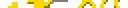
\includegraphics[width=.7\textwidth]{capitulos/capitulo4/new_1d.png}
			\caption{Distribución 1D de los \textit{tiles} en la OAM.}\label{fig:1d}
		\end{figure}

		\begin{figure}[h]
			\centering
			
\includegraphics[width=.4\textwidth]{capitulos/capitulo4/new_2d.png}
			\caption{Distribución 2D de los \textit{tiles} en la OAM.}\label{fig:2d}
		\end{figure}

	\item Bit \{5\}: Al activar este bit, el programador tendrá acceso a la OAM durante HBlank.
	\item Bit \{4\}: Permite la selección del buffer que se muestra por pantalla para los modos 4 y 5, los cuales manejan más de un buffer. Para más información consultar el punto~\ref{sec:mode_4} y~\ref{sec:mode_5}. 
	\item Bit \{3\}: La función que desempeña el tercer bit del registro DISPCNT es mostrar si el juego se está ejecutando en una Game Boy Color. El bit no se puede modificar. 
	\item Bits \{2-0\}: Modo del fondo utilizado. Entre los valores permitidos están el 0, 1 y 2, definidos para las tres maneras que tiene la GBA de procesar fondos. Los modos 3, 4 y 5 están reservados para los fondos bitmap. Los valores 6 y 7 no están permitidos. Las diferencias entre los modos se verán en las secciones~\ref{sec:bitmaps} y~\ref{sec:fondos}.
\end{itemize}

En la Tabla~\ref{tab:dispcnt} se hace un resumen de los parámetros del registro DISPCNT.

\begin{table}[h]
	\centering
	\begin{tabular}{| l | l |}
		\hline
		\textbf{Bits} & \textbf{Función}  \\ \hline
		F & Modo ``ventana'' para \textit{sprites}.  \\ \hline
		E-D & Modo ``ventana'' para fondos.  \\ \hline
		C & Activa el uso de \textit{sprites}.  \\ \hline
		B-8 & Activa cada uno de los 4 fondos disponibles.  \\ \hline
		7 & ``Reset'' de la pantalla.  \\ \hline
		6 & Especifica la distribución de los tiles en memoria. \\ \hline
		5 & Activa el acceso a la OAM durante HBlank. \\ \hline
		4 & Selecciona el buffer adicional en los modos 4 y 5. \\ \hline
		3 & Permite consultar si un juego se está ejecutando en una Game Boy Color. \\ \hline
		2-0 & Selecciona el modo que utiliza la Game Boy Advance para los fondos. \\ \hline
	\end{tabular}
	\caption{Registro \textit{Display Control}.}\label{tab:dispcnt}
\end{table}
\FloatBarrier{}

\subsubsection{DISPSTAT}

El siguiente registro, el \textit{Display Status} (conocido también como el registro DISPSTAT), se sitúa en la dirección de memoria 0x04000004 y permite al programador consultar la información relacionada con el VBlank, HBlank y VCount. VBlank es el período que hay entre cada fotograma refrescado, y HBlank se refiere al período que hay entre cada línea refrescada por pantalla. Por otro lado, VCount es el número de líneas, las filas de píxeles horizontales, refrescadas. Los bits que contiene son los siguientes:
\begin{itemize}
	\item Bits \{F-8\}: El programador especifica un valor VCount determinado, para invocar una interrupción en el bit {5} o que el cambio se vea reflejado en el bit {2}.
	\item Bit \{5\}: Activa la interrupción de VCount si este coincide con el valor especificado en {F-8}.
	\item Bits \{4-3\}: Activa la interrupción de HBlank y VBlank respectivamente.
	\item Bit \{2\}: Este bit tendrá valor si VCount coincide con el valor especificado en {F-8}.
	\item Bits \{1-0\}: Permiten saber si el dispositivo se encuentra en HBlank, si el valor del bit 0 es 1, o en VBlank, si el valor del bit 1 es 1.
\end{itemize}

En la Tabla~\ref{tab:dispstat} se hace un resumen de los parámetros del registro DISPSTAT.

\begin{table}[h]
	\centering
	\begin{tabular}{| l | l |}
		\hline
		\textbf{Bits} & \textbf{Función}  \\ \hline
		F-8 & VCount objetivo.  \\ \hline
		5 & Activa una interrupción al alcanzar VCount objetivo. \\ \hline
		4-3 & Activa la interrupción de HBlank y VBlank. \\ \hline
		2 & Bit activo en caso de alcanzar VCount objetivo.  \\ \hline
		1-0 & Esto de HBlank y VBlank. \\ \hline
	\end{tabular}
	\caption{Registro \textit{Display Status}.}\label{tab:dispstat}
\end{table}
\FloatBarrier{}

El valor de VCount también se puede consultar en la dirección de memoria 0x04000006. Dado que el valor oscila entre 0 y 227, solo se tienen en cuenta los primeros 8 bits.

\subsubsection{Configuración de fondos}\label{sec:conf_fondos}

A continuación, se detallan los registros para controlar los distintos parámetros que pueden tener los fondos de la Game Boy Advance. Estos registros sirven, entre otras cosas, para cambiar el tamaño, color y posicionamiento de los fondos.

\begin{itemize}
	\item Bits \{F-E\}: Tamaño del fondo. Para más información consultar la sección~\ref{sec:fondos}.
	\item Bit {D}: Por defecto, los fondos que no utilizan la matriz de transformación, se repiten en caso de que el \textit{offset} provoque que el fondo llegue a su fin. Este campo permite que los fondos que utilicen la matriz de transformación también se vean repetidos. Para más información, consultar el punto~\ref{sec:fondos}.
	\item Bits \{C-8\}: El índice del grupo de \textit{tiles} especifico que se utiliza.
	\item Bit {7}: Especifica el formato del color a utilizar. Con un 0 se consiguen 16 colores disponibles (4 bpp) y con un 1 se consiguen 256 colores (8 bpp).
	\item Bit {6}: Activa el modo mosaico. Más información en el punto~\ref{sec:sprites}.
	\item Bits \{3-2\}: Especifica el índice del bloque de grupo de \textit{tiles} a utilizar.
	\item Bits \{1-0\}: Prioridad de renderizado del fondo. Cuánto mayor sea el valor antes se renderizará en pantalla. En caso de que haya fondos con la misma prioridad se recurre al orden natural, siendo el primer fondo (BG0) el que mayor prioridad tiene y el último fondo el que menor prioridad tiene (BG3).
\end{itemize}

En la Tabla~\ref{tab:regfondo} se hace un resumen de los parámetros del registro de control de fondos.

\begin{table}[h]
	\centering
	\begin{tabular}{| l | l |}
		\hline
		\textbf{Bits} & \textbf{Función}  \\ \hline
		D & Activar la función ``wrap'' en las matrices que utilicen la matriz de transformación. \\ \hline
		C-8 & El índice del grupo de \textit{tiles} especifico que se utilizará.   \\ \hline
		7 & Rango de colores utilizado.  \\ \hline
		6 & Modo mosaico.  \\ \hline
		3-2 & Especifica el índice del bloque de grupo de \textit{tiles} que se utilizará. \\ \hline
		1-0 & Prioridad de renderizado. \\ \hline
	\end{tabular}
	\caption{Registro de control de fondos.}\label{tab:regfondo}
\end{table}
\FloatBarrier{}

Cada uno de los fondos cuenta con un registro de control específico. La ubicación de los registros para cada fondo se puede observar en la Tabla~\ref{tab:fondo_reg_1}. Además, en la tabla se incluye el \textit{offset} X e Y mencionado anteriormente.

En caso de que el programador quiera renderizar los fondos a través de una matriz de transformación dada (más información en el punto~\ref{sec:ppu}), tiene que configurar los registros de transformación y los registros de referencia. Este último sustituye a los parámetros de \textit{offset} vistos anteriormente para los fondos ``normales'' (aquellos que no utilicen la matriz de transformación).

\begin{table}[h]
	\centering
	\begin{tabular}{| l | l | l | l | l |}
		\hline
		\textbf{Fondos} & \textbf{Registro de Control} & \textbf{Registro de Offset X} & \textbf{Registro de Offset Y}  \\ \hline
		0 & 0x04000008 & 0x04000010 & 0x04000012  \\ \hline
		1 & 0x0400000A & 0x04000014 & 0x04000016  \\ \hline
		2 & 0x0400000C & 0x04000018 & 0x0400001A  \\ \hline
		3 & 0x0400000E & 0x0400001C & 0x0400001E  \\ \hline
	\end{tabular}
	\caption{Registros de cada uno de los fondos (1).}\label{tab:fondo_reg_1}
\end{table}
\FloatBarrier{}

El registro de transformación, como su nombre indica, se limita a almacenar los valores de la matriz de transformación. Los valores de la matriz 2x2 se almacenan consecutivamente, ocupando 2 bytes cada uno, empezando por 0x04000020 para el fondo 2 y 0x04000030 para el fondo 3 (véase la Tabla~\ref{tab:fondo_reg_2}). Estos valores son números \textit{fixed point} desplazados por 8 bits.

\begin{table}[h]
	\centering
	\begin{tabular}{| l | l | l | l | l |}
		\hline
		\textbf{Fondos} & \textbf{Registro de Transformación} & \textbf{Registro de Referencia}  \\ \hline
		0 &  - & -  \\ \hline
		1 & - & -  \\ \hline
		2 & 0x04000028-0x0400002E & 0x04000020-0x04000026  \\ \hline
		3 & 0x04000038-0x0400003E & 0x04000030-0x04000036  \\ \hline
	\end{tabular}
	\caption{Registros de cada uno de los fondos (2).}\label{tab:fondo_reg_2}
\end{table}

El otro registro a tener en cuenta, es el registro de referencia. Este replica el comportamiento del registro de \textit{offset} pero con números \textit{fixed point} de 28 bits. La distribución de los valores es la mostrada en la Tabla~\ref{tab:dist_fixed_fondo}.

\begin{table}[h]
	\centering
	\begin{tabular}{| l | l | l |}
		\hline
		27 & 26--8 & 7--0  \\ \hline
		Signo & Valor entero & Valor decimal  \\ \hline
	\end{tabular}
	\caption{Formato del valor de referencia de los fondos utilizando la matriz de transformación.}\label{tab:dist_fixed_fondo}
\end{table}

Los puntos de referencia X e Y para el fondo 2 se almacenan en las direcciones de memoria 0x04000028 y 0x0400002E respectivamente, mientras que los puntos de referencia X e Y para el fondo 3 se localizan en las direcciones de memoria 0x04000038 y 0x0400003E respectivamente (véase la Tabla~\ref{tab:fondo_reg_2}).

Como se puede apreciar en la Tabla~\ref{tab:fondo_reg_2}, los fondos 0 y 1 no cuentan con la posibilidad de poder utilizar la matriz de transformación.

\subsubsection{Registros de efectos especiales}

Finalmente, en la sección de registros LCD, las tres secciones que quedan son las del modo ventana, modo mosaico y otros efectos especiales. Las demostraciones de estas tres funciones se pueden ver en la Sección~\ref{sec:efectos}.

Dado que se pueden crear dos ventanas diferentes, existen dos registros distintos para cada uno, donde se especifican las dimensiones horizontales y verticales del rectángulo creado. Las dimensiones horizontales se indican en las direcciones 0x04000040 y 0x04000042 para las ventanas 0 y 1 respectivamente. De los 2 bytes que conforman cada valor, se utiliza 1 byte para cada una de las dos coordenadas X que representan las esquinas inferior izquierda y superior derecha del rectángulo. El formato para las coordenadas verticales es exactamente el mismo pero en las direcciones 0x04000044 para la ventana 0 y 0x04000046 para la ventana 1. En caso de que los valores superen la resolución del dispositivo (240x160), el valor introducido se interpreta como el máximo permitido. En el caso de la anchura, 240, y en el caso de la altura, 160. 

Sin embargo, antes de poder configurar las posiciones de las ventanas es necesario especificar cómo funcionan. Para ello se tiene que definir el comportamiento dentro de la ventanas, en el registro WININ en la dirección de memoria 0x04000048, y el comportamiento fuera de estas, en el registro WINOUT en la dirección de memoria 0x0400004A. Los parámetros para WININ son:

\begin{itemize}
	\item Bit \{D\}: Activa efectos especiales como el \textit{blending} y los efectos \textit{fade in} y \textit{fade out} para la ventana 1.
	\item Bit \{C\}: Activa el renderizado de \textit{sprites} para la ventana 1.
	\item Bits \{B-8\}: Activa los fondos 3, 2, 1 y 0, respectivamente, para la ventana 1.
	\item Bit \{5\}: Activa efectos especiales como el \textit{blending} y los efectos \textit{fade in} y \textit{fade out} para la ventana 0.
	\item Bit \{4\}: Activa el renderizado de \textit{sprites} para la ventana 0.
	\item Bits \{3-0\}: Activa los fondos 3, 2, 1 y 0, respectivamente, para la ventana 0.
\end{itemize}

Por otro lado, para controlar lo que se renderizá fuera de la ventana se configuran los siguientes parámetros en WINOUT:

\begin{itemize}
	\item Bit \{D\}: Activa efectos especiales fuera de las ventanas de \textit{sprites}.
	\item Bit \{C\}: Activa el renderizado de \textit{sprites} fuera de una ventana de \textit{sprites}.
	\item Bits \{B-8\}: Activa el renderizado de los fondos 3, 2, 1 y 0, respectivamente, fuera de una ventana de \textit{sprites}.
	\item Bit \{5\}: Activa efectos especiales fuera de las ventana de las de fondo.
	\item Bit \{4\}: Activa el renderizado de \textit{sprites} fuera de una ventana de fondo.
	\item Bits \{3-0\}: Activa el renderizado de los fondos 3, 2, 1 y 0, respectivamente, fuera de las ventanas de fondo.
\end{itemize}

El registro para la función mosaico se encuentra en la dirección de memoria 0x0400004C. El efecto distorsiona (o ``pixela'') la imagen dependiendo del valor que especifique el programador. Para una demostración del efecto consultar la Sección~\ref{sec:efectos}. Los bits que contiene son los siguientes:

\begin{itemize}
	\item Bits \{F-C\}: Distorsión en el eje vertical del \textit{sprite}.
	\item Bits \{B-8\}: Distorsión en el eje horizontal del \textit{sprite}.
	\item Bits \{7-4\}: Distorsión en el eje vertical del fondo.
	\item Bits \{3-0\}: Distorsión en el eje horizontal del fondo.
\end{itemize}

La última región de los registros LCD son aquellos dedicados al renderizado de efectos especiales. En concreto, los que permiten la mezcla de colores (o transparencia) y cambio de intensidad en la representación de los colores\footnote{Un incremento en la intensidad se traduce en una imagen más ``blanca'' mientras que una imagen con menos intensidad se traduce en una imagen más oscura.}.

El principal registro que gestiona toda la configuración relacionada con los efectos especiales es el registro posicionado en 0x04000050, denominado en~\cite{bib:gbatek} como BLDCNT. Los bits que contiene son los siguientes: 

\begin{itemize}
	\item Bits \{D-8\}: Selección de las capas posteriores a mezclar. Cada bit activa el ``backdrop''\footnote{El ``backdrop'' de la GBA consiste en un fondo completamente negro.}, \textit{sprites} y fondos 3, 2, 1 y 0, respectivamente.
	\item Bits \{7-6\}: Selección del efecto a procesar. Siendo 3, se traduce en un incremento en la intensidad de la capa frontal. Si es 2, se hace una disminución en la intensidad de la capa frontal Cuando es 1, se hace una mezcla de colores de las capas frontales con las posteriores seleccionadas. Finalmente, el 0 significa que no se escoge ningún efecto. Para que la mezcla de colores funcione como se espera es necesario que la capa frontal se encuentre, como su nombre indica, por encima de la capa (o capas) posteriores. 
	\item Bits \{5-0\}: Selección de las capas frontales a mezclar. Cada bit activa el ``backdrop'', \textit{sprites} y fondos 3, 2, 1 y 0, respectivamente.
\end{itemize}

Para poder procesar los efectos tal y como desea el programador, este tiene que especificar los valores adecuados en los registros BLDALPHA para configurar el nivel de mezcla entre las capas frontales y posteriores, en 0x0400052. De forma adicional, para controlar el nivel de intensidad en las capas seleccionadas, tendrá que modificar el valor de BLDY en 0x04000054.

En el caso del registro BLDALPHA, que ocupa 2 bytes, los bits \{C-8\} denotan el coeficiente que tendrán las capas posteriores mientras que los bits \{4-0\} indican el coeficiente que tendrán las capas frontales. De forma similar a lo que ocurre con los registros de los fondos que utilizan las matrices de transformación, los 4 bits inferiores de cada coeficiente simbolizan incrementos fraccionales de $1/16$, teniendo cada coeficiente un rango entre 0 y 1. En el caso del registro BLDY, ocurre lo mismo pero solo utilizando los bits \{4-0\} para especificar un valor entre 0 y 1.

\subsection{Registros de sonido}

La Game Boy Advance ofrece 6 modos diferentes de sonido, 4 analógicos y 2 digitales (canales A-B). Hay un registro para controlar cada uno de ellos además de varios generales que controlan el volumen.

El término técnico para referirse a las 6 opciones de la consola para ofrecer audio es ``canal''. Sin embargo, para no confundirlo con los canales de izquierda y derecha, a lo largo del trabajo, se hará referencia a los 6 canales como ``modos''.

La información contenida en esta sección se basa en la documentación oficial~\cite{bib:gba_manual} y en el material adicional disponible en~\cite{bib:belogic}.

\subsubsection{Modos analógicos}
Los dos primeros modos que ofrece el hardware de la consola, los canales 1 y 2, permiten la reproducción de pulsos con la posibilidad de modificar el volumen de cada onda. De forma adicional, el primer modo permite cambiar de dinámicamente la frecuencia de las ondas. Para ello, ambos modos harán uso de registros para modificar el tono y la duración de la onda, teniendo el modo 1 un registro adicional para controlar la frecuencia. 

El registro encargado de la duración, volumen y ciclo de la onda utiliza el siguiente formato para los modos 1 y 2:

\begin{itemize}
	\item Bits \{F-C\}: Volumen inicial del sonido.
	\item Bit \{B\}: Modificación del volumen. 0 para disminuirlo conforme pasa el tiempo y 1 para incrementarlo conforme pasa el tiempo. 
	\item Bits \{A-8\}: El período con el que cambia el volumen. El valor especificado resulta en $n/64$ segundos de período. 
	\item Bits \{7-6\}: El ciclo que toma el pulso. 0 para un ciclo del 12.5\%, 1 para un ciclo del 25\%, 2 para un ciclo del 50\% y 3 para un ciclo del 75\%.
	\item Bits \{5-0\}: La duración del sonido. El valor especificado resulta en $(64-n)/256$ segundos.
\end{itemize}

El registro encargado de la frecuencia de la onda utiliza el siguiente formato para los modos 1 y 2:

\begin{itemize}
	\item Bit \{F\}: En caso de estar activo el bit, ``resetea'' el sonido.
	\item Bit \{E\}: En caso de ser 0, el sonido es reproducido de forma constante. Si es 1, el sonido es reproducido con la duración especificada en los bits \{5-0\} del registro anterior.
	\item Bits \{A-0\}: Frecuencia utilizada para el tono. El valor especificado resulta en $131072/(2048-n)$ Hz.
\end{itemize}

Para indicar un cambio dinámico en la frecuencia, el modo 1 cuenta con el registro ``sweep'', que tiene los siguientes bits:

\begin{itemize}
	\item Bits \{6-4\}: El tiempo que pasa entre cambios de frecuencia. El valor especificado resulta en $n/128$ segundos.
	\item Bit \{3\}: Cómo se modifica la frecuencia. 0 para el incremento con el paso del tiempo y 1 para la disminución.
	\item Bits \{2-0\}: Denota el cambio en la frecuencia. El valor especificado resulta en un cambio en el periodo de $T=T\pm{}T/2^n$. La suma o resta dependerá del valor del bit {3}.
\end{itemize}

En la Tabla~\ref{tab:reg_canal_1_2} se incluyen los registros de los modos 1 y 2.

\begin{table}[h]
	\centering
	\begin{tabular}{| l | l | l | l |}
		\hline
		\textbf{Canal} & \textbf{Registro de duración} & \textbf{Registro de frecuencia} & \textbf{Registro ``sweep''} \\ \hline
		1 & 0x04000062 & 0x04000064 & 0x04000060 \\ \hline
		2 & 0x04000068 & 0x0400006C & - \\ \hline
	\end{tabular}
	\caption{Registros dedicados de los modos 1 y 2.}\label{tab:reg_canal_1_2}
\end{table}
\FloatBarrier{}

El modo 3, permite reproducir ondas almacenadas en el espacio de memoria localizado entre 0x04000090 y 0x0400009F. En este modo se pueden diferenciar los registros de control para la selección, duración y frecuencia.

El primer registro, reservado para seleccionar la muestra localizada en [0x04000090, 0x0400009F] y utilizado para activar el modo, tiene el siguiente formato:

\begin{itemize}
	\item Bit \{7\}: Activa el modo.
	\item Bit \{6\}: Selecciona el grupo a utilizar. Complementa al bit {5}.
	\item Bit \{5\}: En caso de que el valor sea 0, la Game Boy Advance dividirá las ondas almacenadas en el rango de memoria especificado anteriormente en dos grupos diferentes de 32 muestras cada una. En caso de ser 1, gestionará toda la información almacenada en el rango como un solo grupo de 64 muestras.
\end{itemize}

El segundo registro, es el encargado de modificar la duración y el volumen del modo 3:

\begin{itemize}
	\item Bits \{F-D\}: Volumen del modo. 0 para 0\%, 1 para 100\%, 4 para 75\%, 2 para 50\% y 3 para el 25\%.
	\item Bits \{7-0\}: La duración del sonido. El valor especificado resulta en $n/256$ segundos.
\end{itemize}

Finalmente, el tercer registro necesario para utilizar el modo 3 es el encargado de configurar la frecuencia y repetición del sonido. Tiene el mismo formato descrito para los modos 1 y 2, y cuenta con los siguientes bits:

\begin{itemize}
	\item Bit \{F\}: En caso de estar activo el bit, ``resetea'' el sonido.
	\item Bit \{E\}: Si es 0, reproduce el sonido de forma constante. Si es 1, reproduce el sonido con la duración especificada en los bits \{5-0\} del registro anterior.
	\item Bits \{A-0\}: Frecuencia utilizada para el tono. El valor especificado resulta en $131072/(2048-n)$ Hz.
\end{itemize}

El último modo analógico, el modo 4, tiene como función generar ruido como añadido a los demás modos. De los dos registros reservados para el modo, el que controla la duración y el volumen sigue el mismo formato presentado anteriormente. El registro diferente que se introduce en este caso, es el registro de ruido, que tiene la siguiente estructura:

\begin{itemize}
	\item Bit \{F\}: En caso de estar activo el bit, ``resetea'' el sonido.
	\item Bit \{E\}: Si es 0, reproduce el sonido de forma constante. Si es 1, reproduce el sonido con la duración especificada en los bits \{5-0\} del registro anterior.
	\item Bits \{7-4\}: Denota la función a utilizar con la frecuencia especificada en los bits \{2-0\}. La salida de la función (o \textit{pre-scaler divider} como se llama en~\cite{bib:belogic}) será utilizada para generar el ruido. El efecto del valor del campo sobre la función se puede observar en la ecuación~\ref{eq:fn_canal_4}.

	\begin{align}
		Q/2^{valor+1}
		\label{eq:fn_canal_4}
	\end{align}

	\item Bit \{3\}: Controla el período del ruido generado. Si es 0, el periodo es de 127 ciclos y si es de 1, el periodo es de 32767 ciclos.
	\item Bits \{2-0\}: Frecuencia utilizada en conjunto con la función denotada en [7-4] para generar ruido. Las frecuencias vinculadas a los 8 valores disponibles se pueden observar en la Tabla~\ref{tab:frec_canal_4}.

	\begin{table}[h]
		\centering
		\begin{tabular}{| l | l |}
			\hline
			\textbf{Valor} & \textbf{Frecuencia (en MHz)}  \\ \hline
			0 & $4.19304/2$ \\ \hline
			1 & $4.19304/8$ \\ \hline
			2 & $4.19304/16$ \\ \hline
			3 & $4.19304/24$ \\ \hline
			4 & $4.19304/32$ \\ \hline
			5 & $4.19304/40$ \\ \hline
			6 & $4.19304/48$ \\ \hline
			7 & $4.19304/56$ \\ \hline
		\end{tabular}
		\caption{Frecuencias disponibles para generar ruido en el modo 4.}\label{tab:frec_canal_4}
	\end{table}
	\FloatBarrier{}
\end{itemize}

\subsubsection{Modos digitales}
Se introdujeron dos nuevos modos con respecto al sistema de audio de la Game Boy Color. Estos modos, denominados A y B, hacen uso de los dos DACs (Conversor Digital Analógico) de 8 bits incorporados en la consola. Para utilizarlos se distinguen dos tipos de registros, aquellos reservados para indicar los datos a usar y otros para configurar los modos, los registros de control.

Los registros de datos de los modos A y B, se encuentran en las regiones 0x040000A0 y 0x040000A4, respectivamente. El sistema que implementa la Game Boy Advance, denominado Direct Sound, coge los primeros datos que encuentra en el buffer (FIFO), es decir, los 8 bits menos significativos del registro de 32 bits, que serán los primeros en reproducirse. Para activar la salida de sonido de estos modos, y también los modos 1-4, se utilizan tres registros de control. El primero está en 0x04000080 y tiene como función activar y controlar de forma global el volumen de los modos 1-4. Tiene el siguiente formato:

\begin{itemize}
	\item Bits \{F-C\}: Cada uno de los 4 bits activa el canal izquierdo para los modos 1-4.
	\item Bits \{B-8\}: Cada uno de los 4 bits activa el canal derecho para los modos 1-4.
	\item Bits \{6-4\}: Volumen en el canal izquierdo de los primeros 4 modos.
	\item Bits \{2-0\}: Volumen en el canal derecho de los primeros 4 modos.  
\end{itemize}

El segundo registro de control utilizado es el posicionado en la dirección de memoria 0x04000082. Este modifica el volumen global de los modos 1-4 para los dos canales, además de configurar parámetros relacionados con los modos A y B. Tiene el siguiente formato:

\begin{itemize}
	\item Bit \{F\}: Restablece el buffer de datos FIFO del modo B.
	\item Bit \{E\}: Para poder reproducir sonido en los modos A y B, es necesario utilizar el temporizador 0 o 1. En este campo se especifica cual de los dos temporizadores se utilizará para el modo B.
	\item Bits \{D-C\}: Activa los canales izquierdo (2) y/o derecho (1) del modo B.
	\item Bit \{B\}: Restablece el buffer de datos FIFO del modo A.
	\item Bit \{A\}: Al igual que en el campo {E} se especifica el temporizador a utilizar para el modo A, número 0 o 1.
	\item Bits \{9-8\}: Activa los canales izquierdo (2) y/o derecho (1) del modo A.  
	\item Bit \{3\}: Volumen global del modo B.  
	\item Bit \{2\}: Volumen global del modo A.  
	\item Bits \{1-0\}: Volumen global de los primeros 4 modos. 
\end{itemize}

Finalmente, el registro denominado el ``master switch'' se posiciona en la dirección de memoria 0x04000084. El registro también puede servir para consultar el estado actual en el que se encuentran los modos 1-4. Es importante mencionar que los bits destinados a consultar el estado actual de un modo no pueden ser sobrescritos por el programador.

\begin{itemize}
	\item Bit \{7\}: Permite desactivar todos los modos que ofrece la Game Boy Advance al igualar el campo a 0.
	\item Bits \{3-0\}: Especifica el estado de los modos 4, 3, 2 y 1, respectivamente. Un valor igual a 1 denota que el estado está activo, mientras que el 0 indica lo contrario.
\end{itemize}

\subsection{Registros para \textit{Direct Memory Access}}
La GBA ofrece la posibilidad de copiar datos rápidamente de una dirección de memoria a otra mediante el uso de \textit{Direct Memory Access} (DMA)~\cite{bib:dma_book}.

La consola cuenta con 4 variantes de \textit{DMA} con diferentes prioridades y, por ende, finalidades. El canal número 0 permite realizar transferencias con la máxima prioridad disponible. Los canales 1 y 2 se reservan para las transferencias de sonido a los buffers adecuados. Por último, el canal 3 se reserva para transferencias generales.

Los registros de 32 bits que permiten llevar a cabo estas operaciones son los registros fuente, destino y de control \textit{DMA}. Estos tres registros se repiten para cada uno de los 4 canales. En concreto, el registro de control \textit{DMA} sigue el formato descrito a continuación:

\begin{itemize}
	\item Bit \{1F\}: Activa una transferencia mediante \textit{DMA}.
	\item Bit \{1E\}: Activa una interrupción en caso de haberse completado la operación. 
	\item Bits \{1D-1C\}: Especifica cuándo debe comenzar la transferencia: 0 de manera inmediata, 1 al entrar en el estado VBlank, 2 al entrar en el estado HBlank y el comportamiento al igualar a 3 dependerá del canal utilizado. Para los canales reservados para audio se empieza la transferencia una vez que se hayan leído los buffers correspondientes. Para el canal 3 se realiza una transferencia antes de que la \textit{PPU} renderice cada línea horizontal de la pantalla~\cite{bib:tonc}.
	\item Bit \{1A\}: Especifica el tamaño del dato a copiar. 0 para 16 bits y 1 para 32 bits. 
	\item Bit \{19\}: Si se ha seleccionado el modo 1 en los bits \{1D-1C\}, se repite la transferencia cada vez que el dispositivo entre en el estado VBlank. En el caso de haber seleccionado el modo 2 en los bits \{1D-1C\}, se repite la transferencia cada vez que el dispositivo entre en el estado HBlank.
	\item Bits \{18-17\}: Definen la modificación de la dirección fuente que se lleva a cabo al completar una copia: 0 para incrementar la dirección fuente, 1 para decrementar la dirección fuente, 2 para dejar la dirección de destino fija y 3 para incrementar la dirección fuente, restableciendo el valor inicial una vez acabada la operación. 
	\item Bits \{16-15\}: La finalidad de estos dos bits es similar a la mostrada en los bits \{18-17\} pero para la dirección destino.
	\item Bits \{0F-00\}: El número de transferencias realizadas en la operación.
\end{itemize}

Los registros de fuente y destino restantes se configuran simplemente igualando el valor del registro a la dirección de memoria correspondiente. La dirección de memoria para canal quedaría tal y como se muestra en la Tabla~\ref{tab:dma}.

\begin{table}[h]
	\centering
	\begin{tabular}{| l | l | l | l |}
		\hline
		\textbf{Canal} & \textbf{Registro fuente} & \textbf{Registro destino} & \textbf{Registro de control}  \\ \hline
		0 &  0x040000B0 & 0x040000B4 & 0x040000B8 \\ \hline
		1 &  0x040000BC & 0x040000C0 & 0x040000C4 \\ \hline
		2 &  0x040000C8 & 0x040000CC & 0x040000D0 \\ \hline
		3 &  0x040000D4 & 0x040000D8 & 0x040000DC \\ \hline
	\end{tabular}
	\caption{Registros fuente, destino y de control de \textit{DMA}.}\label{tab:dma}
\end{table}
\FloatBarrier{}

Las transferencias que utilizan \textit{DMA}, a pesar de ser más rápidas que las funciones \textit{memcpy} y \textit{memset} convencionales, traen consigo problemas adicionales que pueden causar un comportamiento inesperado. Por ejemplo, al poner a la CPU en un estado ``inerte'', cualquier tipo de interrupción configurada se puede ver afectada~\cite{bib:tonc}.

Finalmente, es importante comentar que el canal 0 únicamente puede copiar desde la RAM interna del dispositivo.

\subsection{Registros de temporización}
La Game Boy Advance ofrece la posibilidad de configurar hasta 4 contadores independientes que permitan un seguimiento del tiempo. Los dos tipos de registros que se diferencian en esta sección, son los registros de control y de datos. Cada uno ocupa 2 bytes~\cite{bib:tonc}. 

El registro de control tiene el siguiente formato:

\begin{itemize}
	\item Bit \{7\}: Activa el temporizador.
	\item Bit \{6\}: Activa la interrupción cuando el temporizador sobrepasa el límite. 
	\item Bit \{2\}: Hace que los ``overflows'' de temporizadores posicionados previamente en memoria incrementen el valor del temporizador. Por ejemplo, si el valor objetivo se alcanza en el temporizador 2, el temporizador 3 incrementará su valor. 
	\item Bits \{1-0\}: Define la frecuencia con la que se actualiza el contador: 0 para una frecuencia de 16.78 MHz, 1 para 262.21 KHz, 2 para 65.536 KHz y 3 para 16.384 KHz. El programador puede conseguir de manera exacta la frecuencia con la que se actualizan los valores especificando un ``offset'' en el registro de datos~\cite{bib:tonc}.
\end{itemize}

El registro de datos complementa al registro de control y permite tanto la lectura del valor actual del contador como la escritura del valor inicial del contador. El valor que provocará el ``overflow'' viene dado por la ecuación~\ref{eq:eq_temporizador}. Dado que el programador puede especificar un valor inicial, no siempre se producirá un ``overflow'' a los 65536 incrementos.

\begin{align}
	65536 - n_{inc} = 0
	\label{eq:eq_temporizador}
\end{align}

El formato de ambos registros se utiliza repetidamente para cubrir cada uno de los 4 temporizadores. Las direcciones de memoria de los registros de control y de datos para cada temporizador se pueden observar en la Tabla~\ref{tab:temporizadores}.

\begin{table}[h]
	\centering
	\begin{tabular}{| l | l | l |}
		\hline
		\textbf{Temporizador} & \textbf{Registro de Control} & \textbf{Registro de Datos}  \\ \hline
		0 &  0x04000102 & 0x04000100  \\ \hline
		1 &  0x04000106 & 0x04000104  \\ \hline
		2 &  0x0400010A & 0x04000108  \\ \hline
		3 &  0x0400010E & 0x0400010C  \\ \hline
	\end{tabular}
	\caption{Registros de control y datos de los temporizadores.}\label{tab:temporizadores}
\end{table}
\FloatBarrier{}

\subsection{Registros de comunicación serie}
La Game Boy Advance permite el intercambio de información con otras GBAs a partir del puerto serie que trae cada una de sus tres variantes. En concreto, la consola ofrece 6 modos diferentes en los que otro dispositivo puede interactuar con la consola. Sin embargo, en este apartado solo se comentarán brevemente el modo normal, que permite la comunicación bidireccional entre dos consolas y unidireccional entre varias GBA; y el modo multijugador, el cual permite la comunicación bidireccional entre un máximo de 4 consolas Game Boy Advance.

Tanto el modo normal como el multijugador precisa del registro de control general de comunicación (llamado RCNT según \cite{bib:gbatek}) y el registro de control de entrada y salida serie (SIOCNT).

En los dos modos es necesario inicializar el registro RCNT (posicionado en la dirección de memoria 0x04000134) a los valores mostrados a continuación:

\begin{itemize}
	\item Bit \{F\}: Su valor debe ser 0 para poder utilizar cualquiera de los dos modos de comunicación.
	\item Bit \{E\}: A pesar de no tener un uso (por lo menos documentado) su valor debe ser 0.
	\item Bits \{8-4\}: A pesar de no tener un uso (por lo menos documentado) su valor debe ser 0.
	\item Bits \{3-0\}: Es irrevelante para los modos descritos en esta sección.
\end{itemize}

El registro SIOCNT, en el que sí hay diferencias entre los dos modos, se ubica en la dirección de memoria 0x04000128. Para el modo normal, el registro sigue el siguiente formato:

\begin{itemize}
	\item Bit \{E\}: Activa la interrupción de comunicación serie en caso de haberse completado una transferencia.
	\item Bit \{D\}: Se hace 0 para activar la comunicación en modo normal y 1 para activar la comunicación en modo multijugador.
	\item Bit \{C\}: El campo configura el tamaño de la transferencia, 0 para 8 bits y 1 para 32 bits.
	\item Bit \{7\}: Especifica el estado actual de la comunicación, 0 denota un estado inactivo y 1 un estado activo.
	\item Bit \{3\}: Estado de salida de datos.
	\item Bit \{2\}: Estado de entrada de datos. Se traduce en el estado del bit \{3\} de los demás dispositivos.
	\item Bit \{1\}: Define la frecuencia a la que funciona la comunicación. Es 0 para 256 KHz y 1 para 2 MHz. Para conseguir estabilidad en la transferencia de datos se recomienda una frecuencia de 256 KHz dado que la transferencia a 2 MHz se reserva para hardware especial \cite{bib:gbatek}.
	\item Bit \{0\}: Indica el reloj utilizado como referencia para la transferencia. Es 0 para el reloj externo y 1 para el interno.
\end{itemize}

El modo multijugador sigue un formato parecido excepto por los valores posicionados en el primer byte del registro. Concretamente, se sigue el siguiente formato:

\begin{itemize}
	\item Bit \{E\}: Activa la interrupción de la comunicación serie en caso de haberse completado una transferencia.
	\item Bit \{D\}: Se hace 0 para activar la comunicación en modo normal y 1 para activar la comunicación en modo multijugador.
	\item Bit \{C\}: Para poder utilizar el modo multijugador el valor debe ser 0.
	\item Bit \{7\}: Especifica el estado actual de la comunicación. Se pone a 0 para indicar un estado inactivo y a 1 para un estado activo. En el caso del modo multijugador, este bit no se puede modificar en los dispositivos esclavos conectados a la GBA principal.
	\item Bit \{6\}: El valor es 1 en caso de haberse producido un error.
	\item Bits \{5-4\}: El valor define el rol que toma el dispositivo en la comunicación. Es 0 para el dispositivo principal, y 1, 2 y 3 para los dispositivos esclavos.
	\item Bit \{3\}: Estado de la conexión. El valor 0 denota un fallo en la conexión, mientras que el 1 indica que todos los demás dispositivos están listos. 
	\item Bit \{2\}: Es similar a los bits \{5-4\}. Denota si el dispositivo tiene el rol maestro (1) o de esclavo (0).
	\item Bits \{1-0\}: Indica la tasa de baudios a la que se envían los datos. Es 0 para 9600, 1 para 38400, 2 para 57600 y 3 para 115200 bps.
\end{itemize}

Los siguientes registros a tener en cuenta son los encargados de enviar los datos a los diferentes dispositivos.  

En el caso del modo normal se pueden distinguir dos registros, uno dedicado a las transferencias de 8 bits (en la dirección de memoria 0x0400012A) y otro para las transferencias de 32 bits (en la dirección de memoria 0x04000122). En el registro de 8 bits, únicamente se almacenarán los 8 bit menos significativos. Para garantizar el correcto funcionamiento de la comunicación, los dos registros deben contener la información a enviar antes de activar la comunicación serie. Al terminar, la información recibida acaba sustituyendo los datos iniciales escritos en ambos registros.

Por otro lado, el modo multijugador, cuenta con un registro específico para el envío de datos, que reutiliza el registro destinado a transferencias de 8 bits en el modo normal, pero esta vez utilizando completamente los 16 bits del registro. Además, se incluyen registros para recibir los datos de cada uno de los roles en una comunicación serie multijugador. La distribución de estos se puede ver en la Tabla~\ref{tab:mult_modo}.

\begin{table}[h]
	\centering
	\begin{tabular}{| l | l |}
		\hline
		\textbf{Dispositivo} & \textbf{Registro I/O para el modo multijugador} \\ \hline
		0 (Máster) &  0x04000120 \\ \hline
		1 (Esclavo) &  0x04000122 \\ \hline
		2 (Esclavo) &  0x04000124 \\ \hline
		3 (Esclavo) &  0x04000126 \\ \hline
	\end{tabular}
	\caption{Registros I/O para el modo multijugador.}\label{tab:mult_modo}
\end{table}
\FloatBarrier{}

\subsection{Registros de los botones}
El dispositivo ofrece dos formas de obtener la entrada del usuario:

\begin{itemize}
	\item La primera es comprobar directamente el registro KEYINPUT, posicionado en la dirección 0x04000130. Este registro ocupa 2 bytes, aunque solo son útiles los primeros 10 bits. La distribución de los botones de la consola se puede observar en la Tabla~\ref{tab:keypad_reg}. Al consultar los valores del registro es necesario tener en cuenta que un 0 en un bit determinado significa que el botón ha sido pulsado, mientras que un 1 indica lo contrario. \\ \\
	
	\begin{table}[h]
		\centering
		\begin{tabular}{| l | l |}
			\hline
			\textbf{Bit} & \textbf{Botón} \\ \hline
			9 &  L \\ \hline
			8 &  R \\ \hline
			7 &  Abajo (D-pad) \\ \hline
			6 &  Arriba (D-pad) \\ \hline
			5 &  Izquierda (D-pad) \\ \hline
			4 &  Derecha (D-pad) \\ \hline
			3 &  Start \\ \hline
			2 &  Select \\ \hline
			1 &  B \\ \hline
			0 &  A \\ \hline
		\end{tabular}
		\caption{Los botones en el registro KEYINPUT.}\label{tab:keypad_reg}
	\end{table}
	
\item La segunda forma, únicamente recomendada para hacer que el dispositivo salga de un estado de bajo consumo, se basa en el uso de interrupciones. Para ello, el programador tendrá que configurar el registro KEYCNT (véase la Tabla~\ref{tab:keypad_irq_reg}), ubicado en la dirección de memoria 0x04000132. \\ \\

\begin{center}
\begin{longtable}{|p{2cm}|p{9cm}|}
\caption{Los botones en el registro KEYCNT.}\label{tab:keypad_irq_reg} \\

\hline \multicolumn{1}{|p{2cm}|}{\textbf{Bit}} & \multicolumn{1}{p{9cm}|}{\textbf{Función}} \\ \hline 
\endfirsthead

\multicolumn{2}{c}%
{{\bfseries \tablename\ \thetable{}}} \\
\hline \multicolumn{1}{|p{2cm}|}{\textbf{Bit}} &
\multicolumn{1}{p{9cm}|}{\textbf{Función}} \\ \hline 
\endhead
F &  La condición que se debe cumplir para que se active la interrupción. 0 para que se active con tener pulsado uno de los botones activados y 1 para que se active con tener pulsado todos los botones activados. \\ \hline
E &  Activa la interrupción de botones de la Game Boy Advance. \\ \hline
\hline \multicolumn{2}{|r|}{{Continúa en la siguiente página}} \\ \hline
\endfoot
9 &  Se tiene en cuenta el botón L para la interrupción. \\ \hline
8 &  Se tiene en cuenta el botón R para la interrupción. \\ \hline
7 &  Se tiene en cuenta el botón de abajo (D-pad) para la interrupción. \\ \hline
6 &  Se tiene en cuenta el botón de arriba (D-pad) para la interrupción. \\ \hline
5 &  Se tiene en cuenta el botón de izquierda (D-pad) para la interrupción. \\ \hline
4 &  Se tiene en cuenta el botón de derecha (D-pad) para la interrupción. \\ \hline
3 &  Se tiene en cuenta el botón Start para la interrupción. \\ \hline
2 &  Se tiene en cuenta el botón Select para la interrupción. \\ \hline
1 &  Se tiene en cuenta el botón B para la interrupción. \\ \hline
0 &  Se tiene en cuenta el botón A para la interrupción. \\
\hline
\endlastfoot
\end{longtable}
\end{center}
\end{itemize}

\subsection{Registros de interrupciones}
Para activar y utilizar las interrupciones en el dispositivo, el programador precisará de tres registros: IME, IE e IF.

El primero, el registro IME (\textit{Interrupt Master Enable Register}), es el encargado de activar el uso de interrupciones en el sistema. De los 4 bytes que ocupa el registro, solo se utiliza el primer bit, para denotar si se utilizan interrupciones o no.

En caso de activar el uso de interrupciones, el programador tendrá que especificar cuáles hay que utilizar. Para ello tendrá que modificar los valores del registro IE (\textit{Interrupt Enable Register}) para indicar cuáles de las 14 interrupciones disponibles serán utilizadas (véase la Tabla~\ref{tab:irq_ie}).

\begin{center}
\begin{longtable}{|p{2cm}|p{9cm}|}
\caption{Interrupciones disponibles en el sistema.}\label{tab:irq_ie} \\

\hline \multicolumn{1}{|p{2cm}|}{\textbf{Bit}} & \multicolumn{1}{p{9cm}|}{\textbf{Función}} \\ \hline 
\endfirsthead

\multicolumn{2}{c}%
{{\bfseries \tablename\ \thetable{}}} \\
\hline \multicolumn{1}{|p{2cm}|}{\textbf{Bit}} &
\multicolumn{1}{p{9cm}|}{\textbf{Función}} \\ \hline 
\endhead
D &  Activa la interrupción al retirar el cartucho de la consola. \\ \hline
		C &  Activa la interrupción para la detección de los botones especificada en el registro KEYCNT. \\ \hline
\hline \multicolumn{2}{|r|}{{Continúa en la siguiente página}} \\ \hline
\endfoot
		B &  Activa la interrupción al completar la transferencia número 3 a través de DMA. \\ \hline
		A &  Activa la interrupción al completar la transferencia número 2 a través de DMA. \\ \hline
		9 &  Activa la interrupción al completar la transferencia número 1 a través de DMA. \\ \hline
		8 &  Activa la interrupción al completar la transferencia número 0 a través de DMA. \\ \hline
		7 &  Activa la interrupción al completar una transferencia por comunicación serie. \\ \hline
		6 &  Activa la interrupción cuando se sobrepasa el temporizador número 3. \\ \hline
		5 &  Activa la interrupción cuando se sobrepasa el temporizador número 2. \\ \hline
		4 &  Activa la interrupción cuando se sobrepasa el temporizador número 1. \\ \hline
		3 &  Activa la interrupción cuando se sobrepasa el temporizador número 0. \\ \hline
		2 &  Activa la interrupción cuando el valor de VCount objetivo especificado en el registro DISPSTAT es alcanzado. \\ \hline
		1 &  Activa la interrupción cuando se entra en la región HBlank de la pantalla. \\ \hline
		0 &  Activa la interrupción cuando se entra en la región VBlank de la pantalla. \\
\hline
\endlastfoot
\end{longtable}
\end{center}

Sin embargo, una vez provocada la interrupción, el programador tendrá que hacerle saber a la máquina que la interrupción ha sido gestionada exitosamente. El registro donde se realiza esta acción es el IF (\textit{Interrupt Request Flags}), en la dirección de memoria 0x04000202. Siguiendo el mismo formato mostrado en la Tabla~\ref{tab:irq_ie}, se tendrá que escribir un 1 en el bit de la interrupción gestionada. Todo esto se hace desde la función que el programador tendrá que especificar en la dirección de memoria 0x03007FFC.
